\documentclass[11pt,a4paper]{article}

\usepackage{main}
\usepackage{evaluation}

\renewcommand{\typedocument}{Évaluation}
\renewcommand{\classe}{6e}
\renewcommand{\titre}{Interrogation et Rattrapage -- Energie et Mouvement}

\begin{document}

\identiteeleve

\creertitre{\titre}

\vspace*{-1em}

\begin{center}
\textit{Durée : 45 minutes -- Calculatrice autorisée \\ Tous les exercices sont à faire sur l'énoncé.}
\end{center}

\vspace*{-1em}

\exercice[7]{Questions de cours - Energie}

\question[1.5]{Citer trois formes d'énergie.}

\vspace{0.8em}

\dotfill\par

\question[1.5]{Donner la définition d'une source d'énergie non-renouvelable.}

\vspace{0.8em}

\dotfill\par\vspace{0.8em}

\dotfill\par

\question[1]{Citer deux exemples de sources d'énergie renouvelable.}

\vspace{0.8em}

\dotfill\par

\question[3]{Cocher la ou les bonnes réponses :}

\vspace{0.5em}
\begin{center}
\renewcommand{\arraystretch}{2}
\begin{tabular}{|p{7cm}|c|c|c|}
\hline
Un convertisseur \ldots{} de l'énergie. & $\square$ crée & $\square$ reçoit & $\square$ fournit \\[6pt]
\hline
L'uranium est une source d'énergie \ldots & $\square$ fossile & $\square$ qui émet beaucoup de CO$_2$ & $\square$ non-renouvelable \\[6pt]
\hline
En physique, on peut parler d'énergie \ldots & $\square$ mécanique & $\square$ verte & $\square$ musculaire \\[6pt]
\hline
\end{tabular}
\end{center}

\exercice[3]{Conversion d'énergie}

Dans un jardin, une fontaine à eau est alimentée par un panneau solaire.
Le panneau capte la lumière du soleil et produit de l'électricité, qui alimente une pompe faisant circuler l'eau.
A chaque étape, de l'énergie thermique est perdue.

\question[3]{Compléter la chaîne énergétique ci-dessous en remplaçant les pointillés par les bonnes réponses.}

\begin{center}
    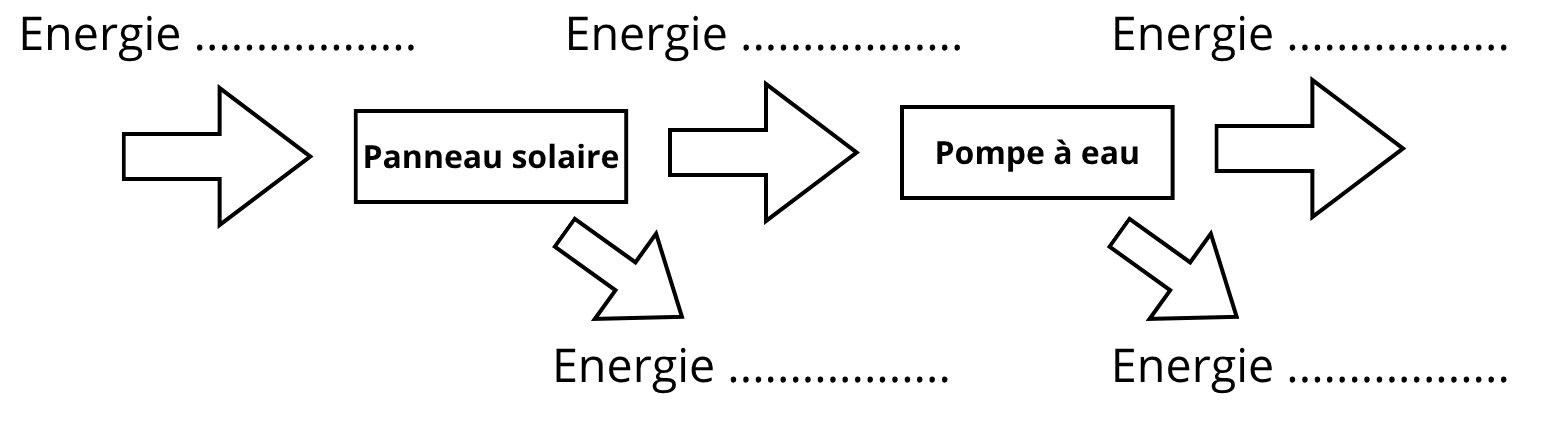
\includegraphics[width=16cm]{images/WE_chaine_energetique.png}
\end{center}

\newpage

\exercice[4]{Questions de cours - Mouvement}

\question[1]{Donner la définition d'un référentiel.}

\vspace{0.8em}
\dotfill\par
\vspace{0.8em}
\dotfill\par


\question[1.5]{Donner la définition d'un mouvement rectiligne uniforme.}

\vspace{0.8em}
\dotfill\par
\vspace{0.8em}
\dotfill\par

\question[1.5]{Donner la formule de la vitesse avec les grandeurs et les unités.}

\vspace{0.8em}
\dotfill\par
\vspace{0.8em}
\dotfill\par

\exercice[6]{Vitesse}

Calculer les grandeurs suivantes en utilisant la formule de la vitesse et en détaillant les calculs:

\question[2]{Le faucon pélerin peut atteindre une vitesse de 110 m/s en piqué. Quelle distance parcourt-il en 5 secondes à cette vitesse ?}

\vspace{0.8em}
\dotfill\par
\vspace{0.8em}
\dotfill\par
\vspace{0.8em}
\dotfill\par

\question[2]{Le tunnel sous la Manche a une longueur de 50 km. L'Eurostar parcourt cette distance en 30 minutes. Quelle est sa vitesse moyenne en km/h ?}

\vspace{0.8em}
\dotfill\par
\vspace{0.8em}
\dotfill\par
\vspace{0.8em}
\dotfill\par

\question[2]{La joueuse de tennis Coco Goff peut lancer une balle à une vitesse de 55 m/s au service. Sachant que la balle parcourt une distance de 24 mètres, combien de temps dure le mouvement ?}

\vspace{0.8em}
\dotfill\par
\vspace{0.8em}
\dotfill\par
\vspace{0.8em}
\dotfill\par

\end{document}